\documentclass{article}
\usepackage{pgfplots}


\begin{document}

\begin{tikzpicture}
\def\Xmax{3}    \def\Ymax{3}
\def\X{1}       \def\Y{2}
\begin{axis}[
	width=8cm,  height=8cm,
	scale only axis=true,
	%
	xmin=-\Xmax,   xmax=\Xmax,
	ymin=-\Ymax,   ymax=\Ymax,
	%
	extra x ticks={-\X,\X},
	extra y ticks={-\Y,\Y},
	extra tick style={grid=major},
]
	\draw[black] (axis cs:0,0)
		ellipse [          x radius=transformdirectionx(\X),y radius=transformdirectiony(\Y)];
	\draw[red]   (axis cs:0,0)
		ellipse [rotate=90,x radius=transformdirectionx(\X),y radius=transformdirectiony(\Y)];
	\addplot [only marks,mark=*] coordinates { (0,0) };
\end{axis}
\end{tikzpicture}

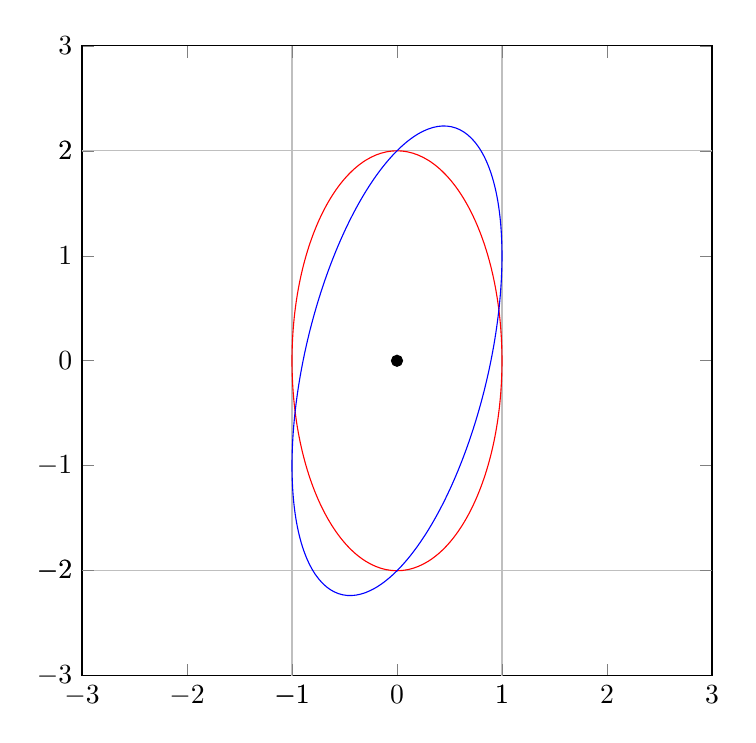
\begin{tikzpicture}
\def\Xmax{3}    \def\Ymax{3}
\def\X{1}       \def\Y{2}
\begin{axis}[
	width=8cm,  height=8cm,
	scale only axis=true,
	%
	xmin=-\Xmax,   xmax=\Xmax,
	ymin=-\Ymax,   ymax=\Ymax,
	%
	extra x ticks={-\X,\X},
	extra y ticks={-\Y,\Y},
	extra tick style={grid=major},
]
	\draw[red]
		\pgfextra{
			\pgfpathellipse{\pgfplotspointaxisxy00}
				{\pgfplotspointaxisdirectionxy{\X}{0}}
				{\pgfplotspointaxisdirectionxy{0}{\Y}}
		};
	\draw[blue]
		\pgfextra{
			\pgfpathellipse{\pgfplotspointaxisxy00}
				{\pgfplotspointaxisdirectionxy{1}{1}}
				{\pgfplotspointaxisdirectionxy{0}{2}}
		};
	\addplot [only marks,mark=*] coordinates { (0,0) };
\end{axis}
\end{tikzpicture}
\end{document}
